\chapter{Комплексные числа}\label{chap:c23-complex}\markright{Глава 34}
\section{От пары координат к новому числу}
\par\addvspace{5pt}\begin{lrbox}{\CatFlowBox}\begin{minipage}[t]{\linewidth}
\setlength{\parskip}{5pt}\setlength{\columnsep}{4.5mm}\setlength{\intextsep}{0pt}
\begin{wrapfigure}[10]{r}{54mm}

\includegraphics[width=54mm,height=58mm,keepaspectratio]{images/unique/art-73.png}
\end{wrapfigure}
Уравнение \(x^2+1=0\) не имеет действительных решений. Вместо изменения правил действительной арифметики построим большее множество, в котором такое уравнение разрешимо. Начнём с конкретных пар действительных чисел и зададим действия над ними; затем проверим, что эти действия действительно обладают нужными свойствами.
\par\WFclear\end{minipage}\end{lrbox}%
\ifdim\dimexpr\ht\CatFlowBox+\dp\CatFlowBox\relax<64mm\dp\CatFlowBox=\dimexpr64mm-\ht\CatFlowBox\relax\fi%
\noindent\usebox{\CatFlowBox}\par\addvspace{5pt}
\begin{definition}
\term{Комплексное число} (complex number) — упорядоченная пара \((a;b)\) действительных чисел. Множество всех таких пар обозначают \(\mathbb C\). Сложение и умножение задаются формулами
\[
(a;b)+(c;d)=(a+c;b+d),
\]
\[
(a;b)(c;d)=(ac-bd;ad+bc).
\]
Действительное число \(a\) отождествляют с парой \((a;0)\). \term{Мнимая единица} (imaginary unit) — число \(i=(0;1)\).
\end{definition}
По определению \(i^2=(0;1)(0;1)=(-1;0)=-1\). Для действительных чисел новые действия сохраняют старые значения: \((a;0)+(c;0)=(a+c;0)\), \((a;0)(c;0)=(ac;0)\). Поэтому действительные числа входят в комплексные с привычными сложением и умножением.

\begin{definition}
\term{Алгебраическая форма} (Cartesian form; algebraic form) комплексного числа — запись \(z=a+bi\), где \(a,b\in\mathbb R\). Здесь \(a+bi=(a;0)+(b;0)i=(a;b)\). Числа \(a=\operatorname{Re}z\) и \(b=\operatorname{Im}z\) называют соответственно \term{действительной частью} (real part) и \term{мнимой частью} (imaginary part).
\end{definition}
Мнимая часть — действительное число \(b\), а не произведение \(bi\). Равенство комплексных чисел означает равенство обеих частей:
\[
a+bi=c+di\quad\Longleftrightarrow\quad a=c,\quad b=d.
\]
Число действительно ровно тогда, когда его мнимая часть равна нулю. При вычислении произведения можно раскрывать скобки и заменять \(i^2\) на \(-1\); именно так получится уже заданная формула умножения пар. Например,
\[
(2+3i)^2=4+12i+9i^2=-5+12i.
\]

\begin{theorem}[Поле комплексных чисел]\label{thm:legacy-c23-1}
Заданные действия превращают \(\mathbb C\) в поле. Ноль равен \((0;0)\), единица — \((1;0)\). Противоположное к \((a;b)\) равно \((-a;-b)\), а обратное к ненулевому \((a;b)\) равно
\[
\left(\frac a{a^2+b^2};-\frac b{a^2+b^2}\right).
\]
\end{theorem}
\begin{proof}
Результаты действий снова являются парами действительных чисел, то есть замкнутость выполнена. Сложение ассоциативно и коммутативно по каждой координате; указанные ноль и противоположный дают абелеву группу по сложению. Для умножения перестановка двух пар не меняет ни \(ac-bd\), ни \(ad+bc\), поэтому оно коммутативно. Умножение на \((1;0)\) сохраняет обе координаты.

Проверим ассоциативность умножения для \((a;b),(c;d),(e;f)\). В обеих расстановках скобок действительная координата после раскрытия равна
\[
ace-bde-adf-bcf,
\]
а мнимая — \(acf-bdf+ade+bce\). Значит, результаты совпадают. Для распределительности умножение \((a;b)\) на сумму двух других пар даёт координаты
\[
a(c+e)-b(d+f)=(ac-bd)+(ae-bf),
\]
\[
a(d+f)+b(c+e)=(ad+bc)+(af+be).
\]
Это сумма соответствующих произведений. Второй распределительный закон следует из коммутативности умножения.

Если \((a;b)\ne(0;0)\), то \(a^2+b^2>0\). Произведение с указанной обратной парой имеет действительную часть \(\frac{a^2+b^2}{a^2+b^2}=1\) и мнимую часть \(\frac{-ab+ba}{a^2+b^2}=0\). Оно равно единице в обоих порядках. Наконец, ноль и единица различны. Все аксиомы поля из предыдущей главы проверены.
\end{proof}
В частности, в \(\mathbb C\) допустимы сокращение ненулевого множителя и свойство нулевого произведения. Если \(zw=0\), то \(z=0\) или \(w=0\). Эти правила следуют из уже доказанных свойств любого поля, а не из изображения точек на рисунке.

\begin{theorem}[Невозможность порядка, согласованного с полем]\label{thm:legacy-c23-2}
На \(\mathbb C\) нельзя задать строгий линейный порядок, который продолжает обычный порядок на \(\mathbb R\), сохраняется при прибавлении одного и того же числа к обеим сторонам и делает произведение двух положительных чисел положительным.
\end{theorem}
\begin{proof}
Предположим, что такой порядок существует. Поскольку \(i\ne0\), по свойству линейного порядка либо \(i>0\), либо \(i<0\). В первом случае произведение положительных \(i\) и \(i\) должно быть положительным, то есть \(-1=i^2>0\). Во втором случае прибавление \(-i\) к \(i<0\) даёт \(0<-i\); снова произведение положительных чисел \((-i)(-i)=i^2=-1\) должно быть положительным. Оба случая противоречат \(-1<0\), унаследованному от действительных чисел.
\end{proof}
Таким образом, привычные сравнения положительности и неотрицательности нельзя автоматически переносить на комплексные числа. Например, утверждение о неотрицательности любого действительного квадрата не даёт ограничения \(z^2\ge0\) для комплексного \(z\). Модули же являются действительными неотрицательными числами, поэтому их сравнивать можно.

\par\addvspace{5pt}\begin{lrbox}{\CatFlowBox}\begin{minipage}[t]{\linewidth}
\setlength{\parskip}{5pt}\setlength{\columnsep}{4.5mm}\setlength{\intextsep}{0pt}
\begin{wrapfigure}[12]{l}{54mm}

\includegraphics[width=54mm,height=58mm,keepaspectratio]{images/unique/art-74.png}
\end{wrapfigure}
Переход от действительных чисел к комплексным расширяет набор допустимых значений, но не отменяет необходимость проверять условия действий. Деление по-прежнему требует ненулевого знаменателя, а равенство требует совпадения обеих координат. Новое число удобно одновременно понимать как алгебраический объект и как пару действительных координат. Первая точка зрения помогает раскрывать скобки и решать уравнения, вторая позволяет независимо проверять результат. Если после преобразований получено одно вещественное уравнение вместо двух, полезно выяснить, не была ли потеряна часть исходного условия. Например, равенство модулей является лишь необходимым условием равенства чисел: оно сохраняет расстояние до начала координат, но не определяет направление. Выбор подходящей формы записи зависит от задачи; надёжное решение сохраняет возможность вернуться к исходному равенству и проверить обе его части.
\par\WFclear\end{minipage}\end{lrbox}%
\ifdim\dimexpr\ht\CatFlowBox+\dp\CatFlowBox\relax<64mm\dp\CatFlowBox=\dimexpr64mm-\ht\CatFlowBox\relax\fi%
\noindent\usebox{\CatFlowBox}\par\addvspace{5pt}
\section{Сопряжение, модуль и деление}
\begin{definition}
\term{Комплексное сопряжение} (complex conjugation) заменяет \(z=a+bi\) на \(\overline z=a-bi\). \term{Модуль комплексного числа} (modulus; absolute value) определяется равенством
\[
|z|=\sqrt{a^2+b^2}.
\]
Это неотрицательное действительное число. Оно равно нулю только при \(z=0\).
\end{definition}
Например, для \(z=2+3i\) имеем \(\overline z=2-3i\), \(|z|=\sqrt{13}\). Сопряжённое число обычно отличается от противоположного: \(-z=-2-3i\).

\begin{theorem}[Сопряжение и модуль произведения]\label{thm:legacy-c23-3}
Для любых \(z,w\in\mathbb C\)
\[
\overline{z+w}=\overline z+\overline w,\qquad
\overline{zw}=\overline z\,\overline w,\qquad
\overline{\overline z}=z,
\]
\[
z\overline z=|z|^2,\qquad
|\overline z|=|z|,\qquad |zw|=|z|\,|w|.
\]
\end{theorem}
\begin{proof}
Пусть \(z=a+bi\), \(w=c+di\). У сопряжённого суммы обе части равны частям суммы сопряжённых. Далее
\[
\overline{zw}=(ac-bd)-(ad+bc)i=(a-bi)(c-di).
\]
Двукратная смена знака мнимой части возвращает \(z\), а умножение \((a+bi)(a-bi)\) даёт \(a^2+b^2=|z|^2\). Квадрат мнимой координаты при сопряжении не меняется, поэтому модули равны. Наконец,
\[
|zw|^2=zw\overline{zw}
=zw\overline z\,\overline w
=(z\overline z)(w\overline w)=|z|^2|w|^2.
\]
Обе стороны требуемого равенства модулей неотрицательны; извлечение квадратного корня завершает доказательство.
\end{proof}
При \(w\ne0\) отсюда получаем удобные формулы
\[
\frac1w=\frac{\overline w}{|w|^2},\qquad
\frac zw=\frac{z\overline w}{|w|^2},\qquad
\left|\frac zw\right|=\frac{|z|}{|w|}.
\]
Первая проверяется умножением на \(w\); вторая — умножением числителя и знаменателя на \(\overline w\). Для третьей применим модуль к равенству \(z=(\frac zw)w\) и разделим на \(|w|>0\). В алгебраической форме деление сводится к действительному знаменателю:
\[
\frac{a+bi}{c+di}=\frac{(ac+bd)+(bc-ad)i}{c^2+d^2},\qquad c+di\ne0.
\]

\section{Комплексная плоскость, расстояние и аргумент}
\begin{definition}
\term{Комплексная плоскость} (complex plane) — координатная плоскость, точке \((a;b)\) которой соответствует число \(a+bi\). Горизонтальная ось действительная, вертикальная — мнимая. Расстояние между числами \(z,w\) на этой плоскости равно \(|z-w|\).
\end{definition}
Сложение чисел соответствует сложению векторов перемещения. Сопряжение отражает точку относительно действительной оси. Модуль — расстояние до начала координат: формула расстояния \(|z-w|=\sqrt{(\operatorname{Re}z-\operatorname{Re}w)^2+(\operatorname{Im}z-\operatorname{Im}w)^2}\) совпадает с формулой длины вектора из главы \ref{chap:c18}.

\begin{definition}
Для \(z=a+bi\ne0\) число \(\varphi\in\mathbb R\) — \term{аргумент} (argument), если
\[
\cos\varphi=\frac a{|z|},\qquad \sin\varphi=\frac b{|z|}.
\]
Обозначение \(\arg z\) в этой главе означает \emph{множество всех} аргументов:
\[
\arg z=\{\varphi+2\pi k:k\in\mathbb Z\}.
\]
У нуля аргумент не определён. \term{Главный аргумент} (principal argument) \(\operatorname{Arg}z\) — единственный аргумент в промежутке \((-\pi;\pi]\).
\end{definition}
Точка \((\frac a{|z|};\frac b{|z|})\) лежит на единичной окружности, поэтому её угол существует. Один полный оборот равен \(2\pi\); все углы этой точки отличаются на целое число полных оборотов. Это объясняет как неоднозначность аргумента, так и единственность выбранного главного значения. Для отрицательного действительного числа главный аргумент равен \(\pi\), а не \(-\pi\), поскольку левый конец выбранного промежутка исключён. Для \(2+3i\) главный аргумент лежит в первой четверти и равен \(\operatorname{arctg}\frac32\). Один только \(\operatorname{arctg}\frac ba\) без учёта четверти не является общей формулой аргумента.

\begin{definition}
\term{Тригонометрическая форма} (polar form; trigonometric form) ненулевого комплексного числа — запись
\[
z=r(\cos\varphi+i\sin\varphi),\qquad r=|z|>0,\quad\varphi\in\arg z.
\]
\end{definition}
Число \(0\) можно формально записать как \(0(\cos\varphi+i\sin\varphi)\) при любом \(\varphi\), но это не задаёт аргумент нуля: никакого направления у нулевого перемещения нет.

\par\addvspace{5pt}\begin{lrbox}{\CatFlowBox}\begin{minipage}[t]{\linewidth}
\setlength{\parskip}{5pt}\setlength{\columnsep}{4.5mm}\setlength{\intextsep}{0pt}
\begin{wrapfigure}[13]{r}{54mm}

\includegraphics[width=54mm,height=58mm,keepaspectratio]{images/unique/art-75.png}
\end{wrapfigure}
Геометрическая запись разделяет две характеристики числа: расстояние до начала координат и направление луча. При переходе к алгебраической форме они снова соединяются в горизонтальную и вертикальную координаты. В задачах на сложение обычно удобнее складывать именно координаты, потому что длины и углы слагаемых по отдельности не дают длину и угол суммы. Для умножения ситуация меняется: длины перемножаются, а углы складываются, что будет доказано ниже. При записи ответа важно отличать конкретный угол от всего множества аргументов. Выбранное главное значение полезно для единого вида ответа, но после арифметического сложения двух главных значений иногда требуется добавить или вычесть полный оборот. На положение точки это не влияет, зато предотвращает ошибочное утверждение, что главный аргумент произведения всегда равен обычной сумме главных аргументов множителей.
\par\WFclear\end{minipage}\end{lrbox}%
\ifdim\dimexpr\ht\CatFlowBox+\dp\CatFlowBox\relax<64mm\dp\CatFlowBox=\dimexpr64mm-\ht\CatFlowBox\relax\fi%
\noindent\usebox{\CatFlowBox}\par\addvspace{5pt}
\section{Умножение как поворот и растяжение}
\begin{theorem}[Умножение в тригонометрической форме]\label{thm:legacy-c23-4}
Если \(z=r(\cos\alpha+i\sin\alpha)\), \(w=s(\cos\beta+i\sin\beta)\), где \(r,s>0\), то
\[
zw=rs\bigl(\cos(\alpha+\beta)+i\sin(\alpha+\beta)\bigr).
\]
При делении \(w\ne0\) модуль делится на \(s\), а аргумент можно взять равным \(\alpha-\beta\).
\end{theorem}
\begin{proof}
Обоснуем нужные формулы сложения углов геометрически. Поворот на угол \(\beta\) переводит первый единичный координатный вектор в \((\cos\beta;\sin\beta)\), а второй — в \((-\sin\beta;\cos\beta)\): второй получается из первого поворотом на прямой угол против часовой стрелки. Геометрический поворот сохраняет длины, направленные отношения отрезков на одной прямой и параллелограммы. Поэтому он сохраняет умножение вектора на действительное число и сложение векторов по правилу параллелограмма. Образ вектора \((x;y)\) равен
\[
x(\cos\beta;\sin\beta)+y(-\sin\beta;\cos\beta).
\]
Для \((x;y)=(\cos\alpha;\sin\alpha)\) это одновременно точка единичной окружности с углом \(\alpha+\beta\). Сравнение координат даёт
\[
\cos(\alpha+\beta)=\cos\alpha\cos\beta-\sin\alpha\sin\beta,
\]
\[
\sin(\alpha+\beta)=\sin\alpha\cos\beta+\cos\alpha\sin\beta.
\]
Теперь раскроем произведение двух тригонометрических форм, заменим \(i^2\) на \(-1\) и применим эти равенства. Получается указанная формула. У \(\cos\beta+i\sin\beta\) обратное число равно \(\cos\beta-i\sin\beta\), поскольку их произведение — \(1\). Это число имеет угол \(-\beta\); умножение на него и на \(\frac1s\) доказывает правило деления.
\end{proof}
Умножение всех точек на фиксированное ненулевое \(w\) поворачивает лучи на один и тот же угол \(\beta\) и изменяет длины в \(s\) раз. Положительные углы означают поворот против часовой стрелки. В частности, умножение на \(i\) поворачивает на \(90^\circ\): \(i(a+bi)=-b+ai\). Умножение на ноль переводит все точки в начало координат и не является поворотом.

\begin{theorem}[Неравенство треугольника]\label{thm:legacy-c23-5}
Для любых комплексных \(z,w\)
\[
|z+w|\le|z|+|w|.
\]
Равенство выполняется, если одно из чисел нулевой, а при двух ненулевых — ровно когда они лежат на одном луче из начала координат.
\end{theorem}
\begin{proof}
Для любого \(\zeta=u+vi\) имеем \(\operatorname{Re}\zeta=u\le\sqrt{u^2+v^2}=|\zeta|\). Равенство здесь эквивалентно \(v=0\), \(u\ge0\). Раскрывая произведение с сопряжённым, получаем
\[
|z+w|^2=|z|^2+2\operatorname{Re}(z\overline w)+|w|^2
\le |z|^2+2|z|\,|w|+|w|^2.
\]
Извлекаем квадратный корень из неотрицательных сторон. При \(z=0\) или \(w=0\) равенство очевидно. Иначе оно эквивалентно тому, что \(z\overline w\) — положительное действительное число. Тогда \(\frac wz=\frac{\overline{z\overline w}}{|z|^2}\) — положительное действительное число, то есть \(w=tz\) с \(t>0\): точки лежат на одном луче. Обратно, такая запись сразу даёт равенство модулей.
\end{proof}

\section{Целые степени и экспоненциальная запись на мнимой оси}
Натуральная степень комплексного числа — произведение одинаковых множителей. При \(z\ne0\) полагают \(z^0=1\) и \(z^{-n}=\frac1{z^n}\) для натурального \(n\). У нуля положительные целые степени равны нулю; отрицательные и \(0^0\) в этой книге не определены.

\begin{theorem}[Формула Муавра; de Moivre's formula]\label{thm:legacy-c23-6}
Для \(r>0\), \(\varphi\in\mathbb R\) и любого целого \(n\)
\[
\bigl(r(\cos\varphi+i\sin\varphi)\bigr)^n
=r^n\bigl(\cos(n\varphi)+i\sin(n\varphi)\bigr).
\]
\end{theorem}
\begin{proof}
При \(n=0\) обе стороны равны \(1\). Для \(n\ge1\) используем индукцию: умножение результата для \(n\) на исходное число умножает модуль на \(r\) и прибавляет к углу \(\varphi\). Это ровно формула для \(n+1\), а база \(n=1\) задана самой записью. Обратное к исходному числу имеет модуль \(r^{-1}\) и угол \(-\varphi\). Применив доказанный натуральный случай к обратному числу, получаем формулу для отрицательных \(n\).
\end{proof}
Как удобное обозначение \emph{для действительных углов} примем
\[
e^{i\varphi}:=\cos\varphi+i\sin\varphi.
\]
Это \term{экспоненциальная запись} (exponential notation) точки единичной окружности; тригонометрическую форму теперь можно записывать как \(z=re^{i\varphi}\). Доказанное правило умножения даёт \(e^{i\alpha}e^{i\beta}=e^{i(\alpha+\beta)}\), а \(e^{i(\varphi+2\pi)}=e^{i\varphi}\). Здесь мы вводим обозначение на мнимой оси и не строим аналитическую теорию экспоненты от произвольного комплексного аргумента. Комплексный логарифм для вычислений этой главы не нужен.

\section{Все решения уравнения \(z^n=w\)}
\begin{definition}
\term{Комплексный корень степени \(n\)} (complex nth root) из \(w\) — любое комплексное число \(z\), удовлетворяющее \(z^n=w\), где \(n\in\mathbb N\). Требуется различать одно найденное решение и множество всех решений. В отличие от арифметического корня из неотрицательного действительного числа, здесь по умолчанию не выбирается одно выделенное значение.
\end{definition}
\begin{theorem}[Корни комплексного числа]\label{thm:legacy-c23-7}
Если \(w=0\), уравнение \(z^n=w\) имеет единственное решение \(z=0\). Если \(w=R(\cos\theta+i\sin\theta)\ne0\), где \(R>0\), то все его решения — ровно \(n\) различных чисел
\[
z_k=\sqrt[n]{R}\left(\cos\frac{\theta+2\pi k}{n}
+i\sin\frac{\theta+2\pi k}{n}\right),
\qquad k=0,1,\ldots,n-1.
\]
В этой формуле \(\sqrt[n]{R}\) — положительный действительный корень; при \(n=1\) понимаем \(\sqrt[1]{R}=R\).
\end{theorem}
\begin{proof}
Если \(z^n=0\), то \(|z|^n=0\), откуда \(|z|=0\) и \(z=0\). Обратно, нулевое число подходит.

Пусть \(w\ne0\). Формула Муавра сразу проверяет, что каждое указанное \(z_k\) в степени \(n\) даёт \(w\). Если два таких числа совпадают, их углы отличаются на целое число полных оборотов. Поэтому \(\frac{2\pi(k-l)}n=2\pi q\) для целого \(q\); значит, \(k-l=nq\). Но \(|k-l|<n\), так что \(k=l\): числа различны.

Для полноты возьмём любое решение \(z\), которое обязательно ненулевое, и запишем \(z=r(\cos\psi+i\sin\psi)\). Тогда \(r^n=R\), поэтому \(r=\sqrt[n]R\), и \(n\psi=\theta+2\pi m\) для некоторого целого \(m\). Разделим \(m\) с остатком: \(m=nq+k\), где \(0\le k<n\). Получаем \(\psi=\frac{\theta+2\pi k}n+2\pi q\), то есть то же число \(z_k\). Других решений нет.
\end{proof}
Для примера \(z^3=8\) имеем \(R=8\), \(\theta=0\), \(\sqrt[3]R=2\). Углы трёх решений: \(0\), \(\frac{2\pi}{3}\), \(\frac{4\pi}{3}\); сами числа равны
\[
2,\qquad -1+i\sqrt3,\qquad -1-i\sqrt3.
\]
Все они лежат на окружности радиуса \(2\), а соседние углы отличаются на \(\frac{2\pi}3\). Отрицательные углы вместо некоторых положительных описывают те же точки.

\par\addvspace{5pt}\begin{lrbox}{\CatFlowBox}\begin{minipage}[t]{\linewidth}
\setlength{\parskip}{5pt}\setlength{\columnsep}{4.5mm}\setlength{\intextsep}{0pt}
\begin{wrapfigure}[10]{l}{54mm}

\includegraphics[width=54mm,height=58mm,keepaspectratio]{images/unique/art-76.png}
\end{wrapfigure}
При извлечении комплексных корней важно сначала отделить модуль от угла, а затем перечислить все допустимые направления. Одна распространённая ошибка состоит в том, чтобы разделить только один выбранный аргумент на показатель степени и закончить решение. Такой шаг действительно даёт один корень, но обычно пропускает остальные. Другая ошибка — брать бесконечно много индексов и считать их разными ответами: после установленного числа шагов направления повторяются. Полнота ответа требует двух проверок: каждое записанное число должно удовлетворять уравнению, а любое возможное решение должно совпасть с одним из перечисленных. Отдельное рассмотрение нуля тоже существенно: у него нет аргумента, поэтому формулу для ненулевого числа нельзя применять буквально. Геометрический рисунок помогает заметить пропуск или повтор, однако окончательное обоснование даёт доказанная формула и проверка её условий.
\par\WFclear\end{minipage}\end{lrbox}%
\ifdim\dimexpr\ht\CatFlowBox+\dp\CatFlowBox\relax<64mm\dp\CatFlowBox=\dimexpr64mm-\ht\CatFlowBox\relax\fi%
\noindent\usebox{\CatFlowBox}\par\addvspace{5pt}
\section{Квадратные уравнения и сопряжённые корни}
\begin{theorem}[Квадратное уравнение с действительными коэффициентами]\label{thm:legacy-c23-8}
Пусть \(a,b,c\in\mathbb R\), \(a\ne0\), \(D=b^2-4ac\). При поиске решений \(az^2+bz+c=0\) в \(\mathbb C\):
\begin{itemize}[leftmargin=1.5em,itemsep=3pt]
\item если \(D>0\), решения — два действительных числа \(\frac{-b+\sqrt D}{2a}\), \(\frac{-b-\sqrt D}{2a}\);
\item если \(D=0\), единственное значение решения — \(-\frac b{2a}\);
\item если \(D<0\), решения — два различных комплексных числа
\[
z=\frac{-b\pm i\sqrt{-D}}{2a}.
\]
\end{itemize}
Во всех формулах квадратный корень применяется к неотрицательному действительному числу.
\end{theorem}
\begin{proof}
Раскрытие квадрата показывает, что исходное уравнение равносильно \((2az+b)^2=D\); умножение и деление на \(a\ne0\) допустимы. При \(D>0\) разложение \((u-\sqrt D)(u+\sqrt D)=0\), где \(u=2az+b\), даёт \(u=\pm\sqrt D\) по свойству нулевого произведения. При \(D=0\) из \(u^2=0\) следует \(u=0\). При \(D<0\) положим \(s=\sqrt{-D}>0\). Тогда \(u^2=-s^2\), то есть \((u-is)(u+is)=0\), откуда \(u=\pm is\). После решения линейного равенства для \(z\) получаются все указанные значения; подстановка или обратное разложение подтверждает каждое из них.
\end{proof}
Например, \(z^2-4z+13=0\) имеет \(D=-36\) и решения \(2+3i\), \(2-3i\). Утверждение прежней главы о том, что при \(D<0\) нет \emph{действительных} корней, остаётся верным: теперь расширена область поиска, а не изменено значение старого утверждения.

\begin{theorem}[Сопряжённые корни многочлена]\label{thm:legacy-c23-9}
Если многочлен \(P\) имеет действительные коэффициенты и \(P(z)=0\), то \(P(\overline z)=0\).
\end{theorem}
\begin{proof}
Сопряжение сохраняет сумму и произведение и оставляет действительный коэффициент неизменным. По индукции оно сохраняет каждую натуральную степень: \(\overline{z^k}=\overline z^{\,k}\). Поэтому при сопряжении суммы степенных слагаемых и свободного действительного члена получаем \(\overline{P(z)}=P(\overline z)\). Из \(P(z)=0\) следует \(P(\overline z)=\overline0=0\).
\end{proof}
Таким образом, невещественные корни многочлена с действительными коэффициентами появляются сопряжёнными парами. Для уравнений, которые удаётся разложить на множители, свойство нулевого произведения позволяет найти все решения по отдельным множителям. Для уравнений \(z^n=w\) полнота уже доказана специальной теоремой. Общего утверждения о числе корней произвольного комплексного многочлена мы здесь не используем.


\section{Примеры: деление и квадратное уравнение}
\begin{example}Чтобы разделить \(1+2i\) на \(1-i\), умножим числитель и знаменатель на сопряжённое \(1+i\). Получаем \(\frac{(1+2i)(1+i)}{(1-i)(1+i)}=\frac{-1+3i}{2}\). Знаменатель равен квадрату модуля и положителен для любого ненулевого делителя.\end{example}
\begin{example}Уравнение \(z^2+2z+5=0\) равносильно \((z+1)^2=-4\). Поэтому корни \(-1+2i\), \(-1-2i\). Их сумма \(-2\), произведение \(5\), что согласуется с Виетом. Среди действительных чисел решений нет, среди комплексных их два.\end{example}
\par\noindent\begin{minipage}{\linewidth}\section*{Графики}
\begin{center}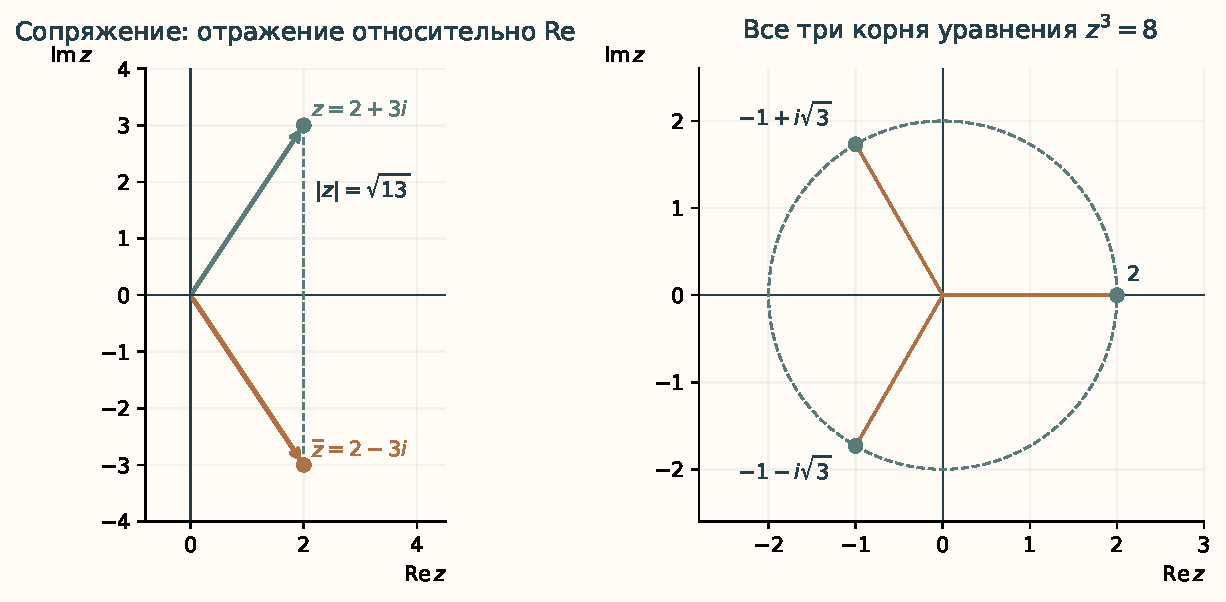
\includegraphics[width=\textwidth,height=.79\textheight,keepaspectratio]{images/atlas-complex.pdf}\par\small Сопряжение и корни на комплексной плоскости\end{center}\end{minipage}\par
\Needspace{7\baselineskip}\section*{Задачи}
\begingroup\setlength{\parskip}{2pt}
\noindent\begin{minipage}[t]{\linewidth}\textbf{34.1.} Используя действия над парами, найди сумму и произведение чисел \((4;-5)\) и \((-2;7)\). Запиши результаты в алгебраической форме.\par\end{minipage}\par
\noindent\begin{minipage}[t]{\linewidth}\textbf{34.2.} Найди все действительные \(a,b\), для которых \((2a-1)+(b+3)i=7-4i\).\par\end{minipage}\par
\noindent\begin{minipage}[t]{\linewidth}\textbf{34.3.} Для \(z=-3+\sqrt2\,i\) укажи \(\operatorname{Re}z\), \(\operatorname{Im}z\) и \(\operatorname{Re}z+i\operatorname{Im}z\). Какие из этих значений являются действительными числами?\par\end{minipage}\par
\noindent\begin{minipage}[t]{\linewidth}\textbf{34.4.} Вычисли \(i^{2027}+i^{2028}\), обосновав сокращение показателей по циклу.\par\end{minipage}\par
\noindent\begin{minipage}[t]{\linewidth}\textbf{34.5.} Для \(z=-8+15i\) найди \(\overline z\), \(-z\), \(|z|\), \(z\overline z\).\par\end{minipage}\par
\noindent\begin{minipage}[t]{\linewidth}\textbf{34.6.} Запиши в алгебраической форме \(\dfrac{7+9i}{2-i}\).\par\end{minipage}\par
\par\addvspace{5pt}\begin{lrbox}{\CatFlowBox}\begin{minipage}[t]{\linewidth}
\setlength{\parskip}{5pt}\setlength{\columnsep}{4.5mm}\setlength{\intextsep}{0pt}
\begin{wrapfigure}[13]{r}{54mm}

\includegraphics[width=54mm,height=58mm,keepaspectratio]{images/unique/art-77.png}
\end{wrapfigure}
\textbf{34.7.} Найди обратное к \(3-4i\) и проверь произведение.\par

\textbf{34.8.} Реши в \(\mathbb C\) линейное уравнение \((2-i)z=4+7i\).\par

\textbf{34.9.} Найди все \(z\), для которых одновременно \(z+\overline z=8\) и \(z-\overline z=-6i\).\par

\textbf{34.10.} Докажи формулы \(\operatorname{Re}z=\dfrac{z+\overline z}{2}\) и \(\operatorname{Im}z=\dfrac{z-\overline z}{2i}\).\par

\textbf{34.11.} Докажи: \(z=\overline z\) тогда и только тогда, когда \(z\) действительно; \(z=-\overline z\) тогда и только тогда, когда \(\operatorname{Re}z=0\). Включён ли ноль во второе утверждение?\par

\textbf{34.12.} Докажи равенства \(|-z|=|z|\) и \(|\overline z|=|z|\), не используя рисунок.\par

\textbf{34.13.} На координатной схеме робот стартует в точке \(1-2i\), затем совершает перемещения \(3+5i\) и \(-2+i\). Найди конечную точку и прямое расстояние от неё до старта.\par
\par\WFclear\end{minipage}\end{lrbox}%
\ifdim\dimexpr\ht\CatFlowBox+\dp\CatFlowBox\relax<64mm\dp\CatFlowBox=\dimexpr64mm-\ht\CatFlowBox\relax\fi%
\noindent\usebox{\CatFlowBox}\par\addvspace{5pt}

\noindent\begin{minipage}[t]{\linewidth}\textbf{34.14.} Найди расстояние и середину отрезка между точками \(z_1=-2+5i\), \(z_2=4-3i\).\par\end{minipage}\par
\noindent\begin{minipage}[t]{\linewidth}\textbf{34.15.} Опиши на комплексной плоскости множество \(\{z:|z-(1-4i)|=3\}\). Укажи центр, радиус и уравнение в координатах \(z=x+yi\).\par\end{minipage}\par
\noindent\begin{minipage}[t]{\linewidth}\textbf{34.16.} Опиши все \(z\), для которых \(\operatorname{Re}z=-2\) и \(|z|\le3\).\par\end{minipage}\par
\noindent\begin{minipage}[t]{\linewidth}\textbf{34.17.} Найди \(\arg(-4i)\) и \(\operatorname{Arg}(-4i)\). Определён ли \(\arg0\)?\par\end{minipage}\par
\noindent\begin{minipage}[t]{\linewidth}\textbf{34.18.} Запиши \(-3+3\sqrt3\,i\) в тригонометрической форме, указав модуль, все аргументы и главный аргумент.\par\end{minipage}\par
\noindent\begin{minipage}[t]{\linewidth}\textbf{34.19.} Пусть \(z=3(\cos\dfrac\pi6+i\sin\dfrac\pi6)\), \(w=4(\cos\dfrac\pi3+i\sin\dfrac\pi3)\). Найди \(zw\) и \(\dfrac zw\) в алгебраической форме.\par\end{minipage}\par
\noindent\begin{minipage}[t]{\linewidth}\textbf{34.20.} В редакторе координат точку \(-1+2i\) сначала поворачивают на \(90^\circ\) по часовой стрелке вокруг нуля, затем увеличивают расстояние до нуля вдвое. Каким множителем задаётся преобразование? Найди новую точку и её расстояние до нуля.\par\end{minipage}\par
\noindent\begin{minipage}[t]{\linewidth}\textbf{34.21.} Точку \(z=4+i\) поворачивают на \(90^\circ\) против часовой стрелки вокруг центра \(c=1+i\). Найди образ. Объясни, почему нужно использовать \(c+i(z-c)\), а не просто \(iz\).\par\end{minipage}\par
\noindent\begin{minipage}[t]{\linewidth}\textbf{34.22.} Докажи, что умножение всех точек на \(i\) сохраняет расстояния: \(|iz_1-iz_2|=|z_1-z_2|\).\par\end{minipage}\par
\noindent\begin{minipage}[t]{\linewidth}\textbf{34.23.} Вычисли \((\sqrt3+i)^6\) с помощью формулы Муавра.\par\end{minipage}\par
\noindent\begin{minipage}[t]{\linewidth}\textbf{34.24.} Вычисли \((1-i)^{-4}\). Объясни, почему отрицательная степень определена.\par\end{minipage}\par
\noindent\begin{minipage}[t]{\linewidth}\textbf{34.25.} Найди все комплексные решения \(z^2=-49\). Есть ли среди них действительные?\par\end{minipage}\par
\noindent\begin{minipage}[t]{\linewidth}\textbf{34.26.} Реши \(z^2+6z+25=0\) в \(\mathbb C\) и укажи сопряжённую пару корней.\par\end{minipage}\par
\noindent\begin{minipage}[t]{\linewidth}\textbf{34.27.} Реши \(z^2+2z-35=0\) в \(\mathbb C\). Объясни, почему переход к комплексным числам не добавляет здесь новых решений.\par\end{minipage}\par
\noindent\begin{minipage}[t]{\linewidth}\textbf{34.28.}\starmark{} Найди все комплексные решения \(z^3=-27\). Запиши их в алгебраической форме и проверь, сколько различных значений получилось.\par\end{minipage}\par
\noindent\begin{minipage}[t]{\linewidth}\textbf{34.29.}\starmark{} Найди все комплексные решения \(z^4=-16\) и опиши их расположение на плоскости.\par\end{minipage}\par
\noindent\begin{minipage}[t]{\linewidth}\textbf{34.30.}\starmark{} Реши в \(\mathbb C\) биквадратное уравнение \(z^4+5z^2+4=0\), найдя все решения.\par\end{minipage}\par
\noindent\begin{minipage}[t]{\linewidth}\textbf{34.31.}\starmark{} Найди все комплексные решения \(z^2=5+12i\), положив \(z=a+bi\) с действительными \(a,b\). Для полноты используй также модуль равенства.\par\end{minipage}\par
\noindent\begin{minipage}[t]{\linewidth}\textbf{34.32.}\starmark{} На координатном плане искомая точка находится на расстоянии \(5\) от начала координат и на расстоянии \(5\) от точки \(6\) действительной оси. Найди все её комплексные координаты и объясни геометрически число ответов.\par\end{minipage}\par
\endgroup
